\documentclass{standalone}
\usepackage{tikz}
\usetikzlibrary{patterns, positioning}


\begin{document}
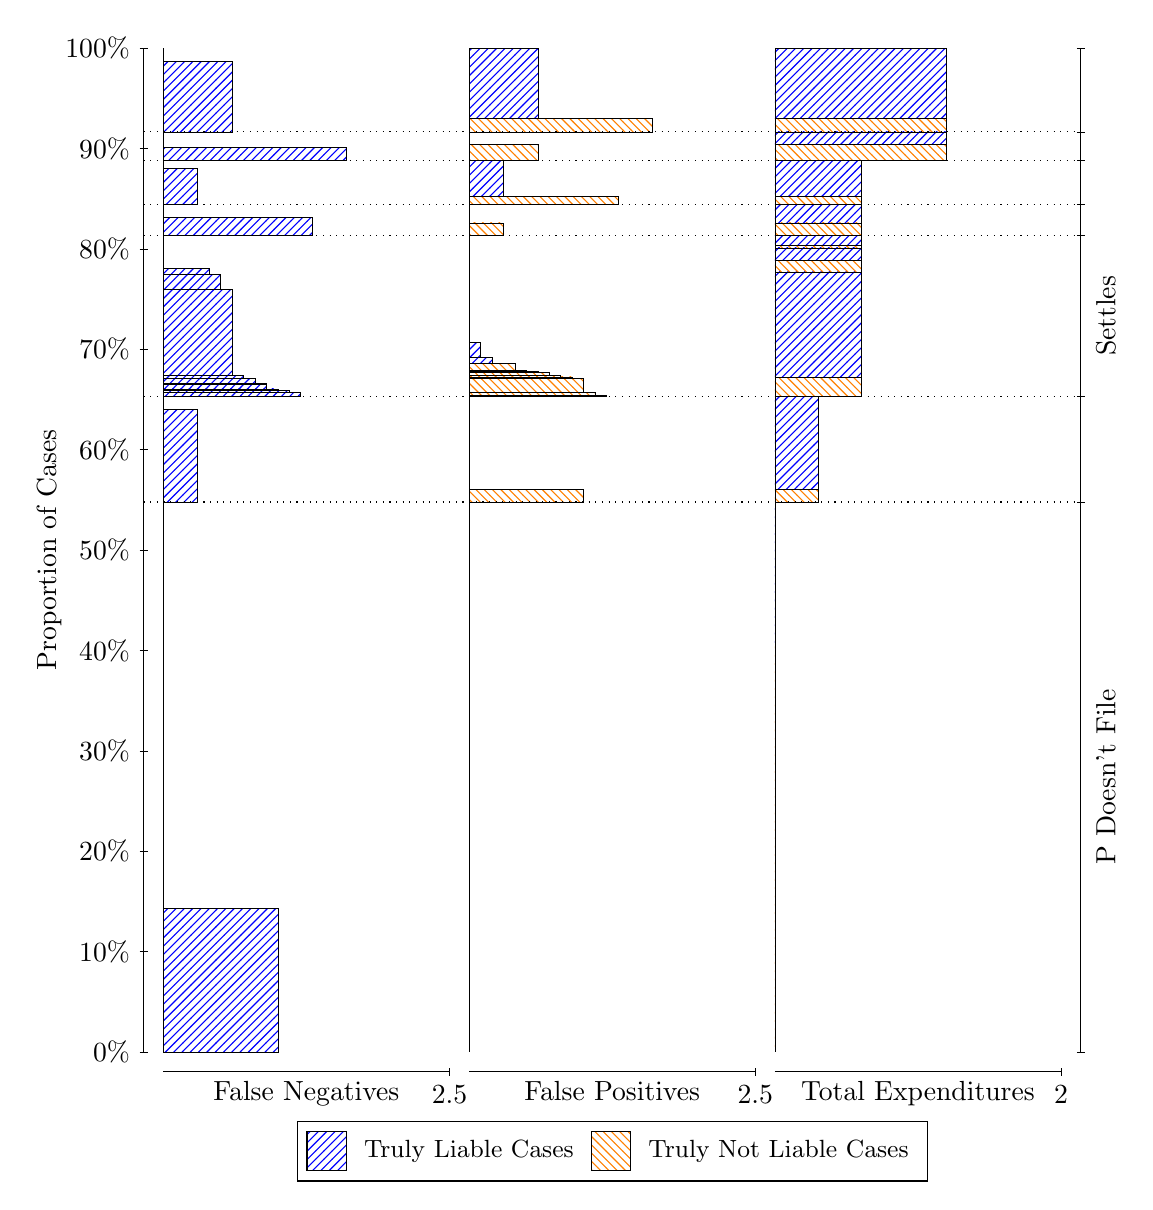
\begin{tikzpicture}
\draw[black, very thin] (1.5,1.75) -- (1.5,14.5);
\node[rotate=90, text=black, anchor=center] at (0.3, 8.125) {Proportion of Cases};
\draw[black, very thin] (1.45,1.75) -- (1.55,1.75);
\node[text=black, anchor=east] at (1.45, 1.75) {0\%};
\draw[black, very thin] (1.45,3.025) -- (1.55,3.025);
\node[text=black, anchor=east] at (1.45, 3.025) {10\%};
\draw[black, very thin] (1.45,4.3) -- (1.55,4.3);
\node[text=black, anchor=east] at (1.45, 4.3) {20\%};
\draw[black, very thin] (1.45,5.575) -- (1.55,5.575);
\node[text=black, anchor=east] at (1.45, 5.575) {30\%};
\draw[black, very thin] (1.45,6.85) -- (1.55,6.85);
\node[text=black, anchor=east] at (1.45, 6.85) {40\%};
\draw[black, very thin] (1.45,8.125) -- (1.55,8.125);
\node[text=black, anchor=east] at (1.45, 8.125) {50\%};
\draw[black, very thin] (1.45,9.4) -- (1.55,9.4);
\node[text=black, anchor=east] at (1.45, 9.4) {60\%};
\draw[black, very thin] (1.45,10.675) -- (1.55,10.675);
\node[text=black, anchor=east] at (1.45, 10.675) {70\%};
\draw[black, very thin] (1.45,11.95) -- (1.55,11.95);
\node[text=black, anchor=east] at (1.45, 11.95) {80\%};
\draw[black, very thin] (1.45,13.225) -- (1.55,13.225);
\node[text=black, anchor=east] at (1.45, 13.225) {90\%};
\draw[black, very thin] (1.45,14.5) -- (1.55,14.5);
\node[text=black, anchor=east] at (1.45, 14.5) {100\%};

\draw[black, very thin] (13.4,1.75) -- (13.4,14.5);
\draw[black, very thin] (13.35,1.75) -- (13.45,1.75);
\node[anchor=west] at (13.35, 1.75) {};
\draw[black, very thin] (13.35,8.7347) -- (13.45,8.7347);
\node[anchor=west] at (13.35, 8.7347) {};
\draw[black, very thin] (13.35,10.079) -- (13.45,10.079);
\node[anchor=west] at (13.35, 10.079) {};
\draw[black, very thin] (13.35,12.117) -- (13.45,12.117);
\node[anchor=west] at (13.35, 12.117) {};
\draw[black, very thin] (13.35,12.512) -- (13.45,12.512);
\node[anchor=west] at (13.35, 12.512) {};
\draw[black, very thin] (13.35,13.072) -- (13.45,13.072);
\node[anchor=west] at (13.35, 13.072) {};
\draw[black, very thin] (13.35,13.436) -- (13.45,13.436);
\node[anchor=west] at (13.35, 13.436) {};
\draw[black, very thin] (13.35,14.5) -- (13.45,14.5);
\node[anchor=west] at (13.35, 14.5) {};

\draw[black, very thin, pattern color=blue, pattern=north east lines] (1.75,1.75) rectangle (3.2033,3.5766);
\draw[black, very thin, pattern color=orange, pattern=north west lines] (1.75,3.5766) rectangle (1.75,8.7347);
\draw[black, very thin, pattern color=blue, pattern=north east lines] (1.75,8.7347) rectangle (2.186,9.9139);
\draw[black, very thin, pattern color=orange, pattern=north west lines] (1.75,9.9139) rectangle (1.75,10.079);
\draw[black, very thin, pattern color=blue, pattern=north east lines] (1.75,10.079) rectangle (3.494,10.129);
\draw[black, very thin, pattern color=blue, pattern=north east lines] (1.75,10.129) rectangle (3.3487,10.148);
\draw[black, very thin, pattern color=blue, pattern=north east lines] (1.75,10.148) rectangle (3.2033,10.172);
\draw[black, very thin, pattern color=blue, pattern=north east lines] (1.75,10.172) rectangle (3.058,10.236);
\draw[black, very thin, pattern color=blue, pattern=north east lines] (1.75,10.236) rectangle (3.058,10.244);
\draw[black, very thin, pattern color=blue, pattern=north east lines] (1.75,10.244) rectangle (2.9127,10.301);
\draw[black, very thin, pattern color=blue, pattern=north east lines] (1.75,10.301) rectangle (2.7673,10.346);
\draw[black, very thin, pattern color=blue, pattern=north east lines] (1.75,10.346) rectangle (2.622,11.438);
\draw[black, very thin, pattern color=blue, pattern=north east lines] (1.75,11.438) rectangle (2.4767,11.629);
\draw[black, very thin, pattern color=blue, pattern=north east lines] (1.75,11.629) rectangle (2.3313,11.7);
\draw[black, very thin, pattern color=orange, pattern=north west lines] (1.75,11.7) rectangle (1.75,12.117);
\draw[black, very thin, pattern color=blue, pattern=north east lines] (1.75,12.117) rectangle (3.6393,12.35);
\draw[black, very thin, pattern color=orange, pattern=north west lines] (1.75,12.35) rectangle (1.75,12.512);
\draw[black, very thin, pattern color=blue, pattern=north east lines] (1.75,12.512) rectangle (2.186,12.967);
\draw[black, very thin, pattern color=orange, pattern=north west lines] (1.75,12.967) rectangle (1.75,13.072);
\draw[black, very thin, pattern color=blue, pattern=north east lines] (1.75,13.072) rectangle (4.0753,13.235);
\draw[black, very thin, pattern color=orange, pattern=north west lines] (1.75,13.235) rectangle (1.75,13.436);
\draw[black, very thin, pattern color=blue, pattern=north east lines] (1.75,13.436) rectangle (2.622,14.334);
\draw[black, very thin, pattern color=orange, pattern=north west lines] (1.75,14.334) rectangle (1.75,14.5);
\draw[black, very thin, pattern color=orange, pattern=north west lines] (5.6333,1.75) rectangle (5.6333,6.9081);
\draw[black, very thin, pattern color=blue, pattern=north east lines] (5.6333,6.9081) rectangle (5.6333,8.7347);
\draw[black, very thin, pattern color=orange, pattern=north west lines] (5.6333,8.7347) rectangle (7.0867,8.8994);
\draw[black, very thin, pattern color=blue, pattern=north east lines] (5.6333,8.8994) rectangle (5.6333,10.079);
\draw[black, very thin, pattern color=orange, pattern=north west lines] (5.6333,10.079) rectangle (7.3773,10.091);
\draw[black, very thin, pattern color=orange, pattern=north west lines] (5.6333,10.091) rectangle (7.232,10.126);
\draw[black, very thin, pattern color=orange, pattern=north west lines] (5.6333,10.126) rectangle (7.0867,10.307);
\draw[black, very thin, pattern color=orange, pattern=north west lines] (5.6333,10.307) rectangle (6.9413,10.323);
\draw[black, very thin, pattern color=orange, pattern=north west lines] (5.6333,10.323) rectangle (6.796,10.345);
\draw[black, very thin, pattern color=orange, pattern=north west lines] (5.6333,10.345) rectangle (6.6507,10.376);
\draw[black, very thin, pattern color=orange, pattern=north west lines] (5.6333,10.376) rectangle (6.5053,10.39);
\draw[black, very thin, pattern color=orange, pattern=north west lines] (5.6333,10.39) rectangle (6.36,10.405);
\draw[black, very thin, pattern color=orange, pattern=north west lines] (5.6333,10.405) rectangle (6.2147,10.496);
\draw[black, very thin, pattern color=blue, pattern=north east lines] (5.6333,10.496) rectangle (5.924,10.567);
\draw[black, very thin, pattern color=blue, pattern=north east lines] (5.6333,10.567) rectangle (5.7787,10.757);
\draw[black, very thin, pattern color=blue, pattern=north east lines] (5.6333,10.757) rectangle (5.6333,12.117);
\draw[black, very thin, pattern color=orange, pattern=north west lines] (5.6333,12.117) rectangle (6.0693,12.28);
\draw[black, very thin, pattern color=blue, pattern=north east lines] (5.6333,12.28) rectangle (5.6333,12.512);
\draw[black, very thin, pattern color=orange, pattern=north west lines] (5.6333,12.512) rectangle (7.5227,12.618);
\draw[black, very thin, pattern color=blue, pattern=north east lines] (5.6333,12.618) rectangle (6.0693,13.072);
\draw[black, very thin, pattern color=orange, pattern=north west lines] (5.6333,13.072) rectangle (6.5053,13.274);
\draw[black, very thin, pattern color=blue, pattern=north east lines] (5.6333,13.274) rectangle (5.6333,13.436);
\draw[black, very thin, pattern color=orange, pattern=north west lines] (5.6333,13.436) rectangle (7.9587,13.602);
\draw[black, very thin, pattern color=blue, pattern=north east lines] (5.6333,13.602) rectangle (6.5053,14.5);
\draw[black, very thin, pattern color=orange, pattern=north west lines] (9.5167,1.75) rectangle (9.5167,6.9081);
\draw[black, very thin, pattern color=blue, pattern=north east lines] (9.5167,6.9081) rectangle (9.5167,8.7347);
\draw[black, very thin, pattern color=orange, pattern=north west lines] (9.5167,8.7347) rectangle (10.062,8.8994);
\draw[black, very thin, pattern color=blue, pattern=north east lines] (9.5167,8.8994) rectangle (10.062,10.079);
\draw[black, very thin, pattern color=orange, pattern=north west lines] (9.5167,10.079) rectangle (10.607,10.317);
\draw[black, very thin, pattern color=blue, pattern=north east lines] (9.5167,10.317) rectangle (10.607,11.656);
\draw[black, very thin, pattern color=orange, pattern=north west lines] (9.5167,11.656) rectangle (10.607,11.804);
\draw[black, very thin, pattern color=blue, pattern=north east lines] (9.5167,11.804) rectangle (10.607,11.961);
\draw[black, very thin, pattern color=orange, pattern=north west lines] (9.5167,11.961) rectangle (10.607,11.993);
\draw[black, very thin, pattern color=blue, pattern=north east lines] (9.5167,11.993) rectangle (10.607,12.117);
\draw[black, very thin, pattern color=orange, pattern=north west lines] (9.5167,12.117) rectangle (10.607,12.28);
\draw[black, very thin, pattern color=blue, pattern=north east lines] (9.5167,12.28) rectangle (10.607,12.512);
\draw[black, very thin, pattern color=orange, pattern=north west lines] (9.5167,12.512) rectangle (10.607,12.618);
\draw[black, very thin, pattern color=blue, pattern=north east lines] (9.5167,12.618) rectangle (10.607,13.072);
\draw[black, very thin, pattern color=orange, pattern=north west lines] (9.5167,13.072) rectangle (11.697,13.274);
\draw[black, very thin, pattern color=blue, pattern=north east lines] (9.5167,13.274) rectangle (11.697,13.436);
\draw[black, very thin, pattern color=orange, pattern=north west lines] (9.5167,13.436) rectangle (11.697,13.602);
\draw[black, very thin, pattern color=blue, pattern=north east lines] (9.5167,13.602) rectangle (11.697,14.5);
\draw[black, dotted] (1.5,8.7347) -- (13.4,8.7347);
\draw[black, dotted] (1.5,10.079) -- (13.4,10.079);
\draw[black, dotted] (1.5,12.117) -- (13.4,12.117);
\draw[black, dotted] (1.5,12.512) -- (13.4,12.512);
\draw[black, dotted] (1.5,13.072) -- (13.4,13.072);
\draw[black, dotted] (1.5,13.436) -- (13.4,13.436);
\draw[black, very thin] (1.75,1.5) -- (5.3833,1.5);
\node[text=black, anchor=north] at (3.5667, 1.5) {False Negatives};
\draw[black, very thin] (5.3833,1.45) -- (5.3833,1.55);
\node[text=black, anchor=north] at (5.3833, 1.45) {2.5};

\draw[black, very thin] (5.6333,1.5) -- (9.2667,1.5);
\node[text=black, anchor=north] at (7.45, 1.5) {False Positives};
\draw[black, very thin] (9.2667,1.45) -- (9.2667,1.55);
\node[text=black, anchor=north] at (9.2667, 1.45) {2.5};

\draw[black, very thin] (9.5167,1.5) -- (13.15,1.5);
\node[text=black, anchor=north] at (11.333, 1.5) {Total Expenditures};
\draw[black, very thin] (13.15,1.45) -- (13.15,1.55);
\node[text=black, anchor=north] at (13.15, 1.45) {2};

\node[text=black, centered, rotate=90] at (13.72, 5.2423) {P Doesn't File};

\node[text=black, centered, rotate=90] at (13.72, 11.098) {Settles};





\draw (7.449999999999999,1.5) node[draw=none] (baseCoordinate) {};
\begin{scope}[align=center]
        \matrix[scale=0.5, draw=black, below=0.5cm of baseCoordinate, nodes={draw}, column sep=0.1cm]{
            \node[rectangle, draw, minimum width=0.5cm, minimum height=0.5cm, pattern color=blue, pattern=north east lines] {}; &
            \node[draw=none, font=\small, text=black] (B) {Truly Liable Cases}; &
            \node[rectangle, draw, minimum width=0.5cm, minimum height=0.5cm, pattern color=orange, pattern=north west lines] {}; &
            \node[draw=none, font=\small, text=black] (B) {Truly Not Liable Cases}; \\
            };
\end{scope}

\end{tikzpicture}
\end{document}